%%%%%%%%%%%%%%%%%%%%%%%%%%%%%%%%%%%%%%%%%%%%%%%%%%%%%%%%%%%%%%%%%%%%%%%%%%%%%%%%%%%%
%% PIPELINE DESIGN
%%%%%%%%%%%%%%%%%%%%%%%%%%%%%%%%%%%%%%%%%%%%%%%%%%%%%%%%%%%%%%%%%%%%%%%%%%%%%%%%%%%%

\begin{table}[!b]
	\centering
	\caption{System Integration and Bounded Overhead.}
	\vspace{-0.31cm} 
    \setlength\tabcolsep{6.62pt}
	\begin{tabular}{l|cc|c}
	  \toprule
		\textbf{Approach} & \textbf{Separation} & \textbf{Reuse} & \textbf{Bounded Overhead} \\
		\midrule
        Eddies    & $\times$ & $\times$ & $\times$ \\
		SkinnerDB & $\times$ & $\times$ & \checkmark \\
        LIP       & (\checkmark) & \checkmark & $\times$ \\
        \midrule
        POLAR     & \checkmark & \checkmark & (\checkmark) \\
		\bottomrule
	\end{tabular}
    %\vspace{-0.1cm}
	\label{tab:comparison}
\end{table}

\section{Pipeline Design}
\label{pipeline-design}
%
% pipeline enhancement, telemetry, parallelism
POLAR is an adaptive join processing approach designed for non-invasive integration into common database systems with support for vectorization and operator pipelining. In contrast to other AQP techniques, POLAR pipelines do not require fine-grained intertwining of existing optimizers and runtime systems. As shown in Figure~\ref{fig:pipeline_design} (right), we enhance amenable pipelines with additional join orders. At runtime, we measure the performance of these orders and route tuples to well-performing orders while exploring others using a regret budget. This section introduces POLAR's design objectives and gives an overview of the compilation and execution of POLAR pipelines and related essential primitives.

\subsection{Design Objectives}
\label{sec:objectives}

We largely attribute the stagnant adoption of adaptive join processing approaches to difficult system integration and problematic performance regressions. Accordingly, we propose a non-invasive approach specifically designed for low and bounded overhead. In the following, we define these objectives and distinguish POLAR from existing AQP systems along these dimensions (in Table \ref{tab:comparison}). As bitmap filtering is increasingly adopted in popular database systems~\cite{DingCN20, LeeDNC23}, we also compare POLAR to Lookahead Information Passing~\cite{ZhuPSP17} (LIP) as a representative candidate. 

\textbf{Non-invasive System Integration:} We call an AQP system non-invasive if it clearly separates compilation from execution (no plan generation at runtime) because this separation simplifies debugging and testing. Furthermore, for simple system integration and maintenance, a non-invasive AQP system should reuse existing infrastructure such as the query optimizer and physical operators. Eddies~\cite{HellersteinA00} and SkinnerDB~\cite{TrummerWMMJA19} intertwine query processing phases, and require specific optimizers and operators. LIP mostly adheres to non-invasiveness but generates new bloom filter orders at runtime.

\textbf{Bounded Overhead:} Preventing major performance regressions on any workload---even if adaptation is not beneficial---is essential for enabling AQP by default. Accordingly, an AQP system should provide bounds for the overhead of adaptivity (e.g., exploration of alternative join orders). Eddies and LIP do not define bounds for their overheads, SkinnerDB gives a strict bound based on the single best (robust) join plan, and POLAR provides a probabilistic bound on the number of intermediates incurred for exploration.

\vspace{-0.1cm}
\subsection{POLAR Pipeline Compilation}
\label{pipeline-enhancement}

%overview 
During query compilation (cf. Figure~\ref{fig:pipeline_design}), we replace amenable operator pipelines with POLAR pipelines. A POLAR pipeline contains alternative join orders and two dedicated operators: a \textit{multiplexer} (for tuple routing) and an \textit{adaptive union} $\cup$ (for result consolidation). In the following, we describe the pipeline selection, the dedicated operators, and the pipeline transformation in more detail.

\textbf{Pipeline Construction:} After query optimization and generation of a query execution plan---consisting of multiple operator pipelines---POLAR replaces all pipelines of left-deep join trees with at least two joins (where the right-hand-sides are build sides, and left-hand-side intermediates are probed in a pipelined fashion). The pipeline's source is the left-most node and fixed as POLAR's source of input tuples for the tuple routing. Our approach generates a set of alternative join orders using a \emph{join order selection} algorithm (cf. Section~\ref{sec:paths}) and includes them with the original join order. Although focusing only on existing join pipelines is limiting, it allows for a system integration without changing the query optimizer and robust performance that is at least as good as the original plan. If the original plan contains pipelines with multiple joins, POLAR can improve these pipelines via alternative orders.

\textbf{Custom Operators:} Additionally, we introduce two new operators into each POLAR pipeline for tuple routing. The \emph{multiplexer} (cf. Section \ref{sec:routing_strategies}) accepts bags of tuples from the source table and determines the next path and the number of tuples to route to that path. It uses performance indicators from previous path runs to make routing decisions. After each path run, a lightweight \emph{adaptive union} operator processes the results from the last join. Besides normal union-all semantics, this operator re-arranges the additional columns from the joins to a consistent order of the original plan.

\textbf{Pipeline Transformation:} Finally, we replace the existing operator pipeline with a POLAR pipeline consisting of the multiplexer, the set of join orders, and the adaptive union. The individual join orders reuse the read-only hash tables of the build sides without redundant allocation. This transformation does not break the pipeline to prevent further materialization and multiplexing. Other non-blocking operators (\eg projections, filters) and the pipeline sink (\eg aggregation) also remain unchanged. The POLAR pipeline allocates space for state per alternative join order (e.g., operator caches, intermediate result vectors). Thus, the space overhead grows linearly with the number of join orders but is negligible in practice.

\vspace{-0.1cm}
\subsection{Join Order Selection}
\label{sec:paths}

When generating alternative join orders for individual pipelines, we aim to compose a diverse set of orders that could handle a wide range of mis-estimated cardinalities and clustered data. The selection strategy should find good plans early (\ie be robust for large pipelines), should not re-invoke the query optimizer (\ie ensure non-invasive integration and low overhead), and should pick few complementary join orders (\ie reduce the amount of exploration overhead). To this end, we propose two novel, anytime join order selection strategies that do not require optimizer invocations, as well as additional heuristics to serve as baselines.

\begin{algorithm}[!t] \small
\caption{Selectivity Space Sampling}\label{alg:enumeration1}
\begin{algorithmic}[1]
\Require{Joins $J$, Max Join Orders $\mathit{MAX}$, Max Iterations $\mathit{maxi}$}
\Ensure{Join Orders $T$}
\State $T \gets \emptyset$, $i \gets 0$
\State $\mat{D} \gets \textsc{discretizeSelectivities}(J)$ \Comment{exponential decay}
\While{$\card{T} < \mathit{MAX} \wedge i < maxi$} 
  \State $d_i \gets \textsc{sample}($\mat{D}$)$, $i \gets i+1$ \Comment{$\card{J}$ selectivities} 
	\State $T \gets T \cup \textsc{DPSize}($J$, d_i)$ \Comment{keep distinct optimal join orders}
\EndWhile
\State \Return $T$
\end{algorithmic}
\end{algorithm}

\begin{algorithm}[!t] \small
\caption{Next-best Join Order Search}\label{alg:enumeration2}
\begin{algorithmic}[1]
\Require{Joins $J$, Edge Counts $n_0, ..., n_{\card{J}} \in N$, Max Join Orders $\mathit{MAX}$}
\Ensure{Join Orders $T$}
\State $R \gets \emptyset$
\State $S \gets \textsc{LegalJoinCandidates}(R, J)$ \Comment{Find first join candidates}
\For{$i \gets 0$ \textbf{to} $n_0$}
    \Comment{Consider $n_0$ of the candidates}
    \State $s_i \gets \textsc{GetNextJoin}(S)$
    \State $\mathit{prio} \gets (\card{R}, i)$
    \State $pqueue.\textsc{Enqueue}(prio, R, s_i)$
    \State $S \gets S \setminus s_i$
\EndFor
\While{$!pqueue.\textsc{Empty}()$ and $\card{J} < \mathit{MAX}$}
    \State $R, s \gets pqueue.\textsc{Dequeue}()$ \Comment{Remove next item}
    \State $R \gets R \oplus s$
    \If{$\card{R} = \card{J} - 1$}
        \State $R \gets R \oplus J \setminus R$ \Comment{Append remaining join}
        \State $T \gets T \cup R$
    \Else
        \State $S \gets \textsc{LegalJoinCandidates}(R, J)$
        \For{$i \gets 0$ \textbf{to} $n_{\card{R}}$}
            \State $s_i \gets \textsc{GetNextJoin}(S)$
            \State $\mathit{prio} \gets (\card{R}, i)$
            \State $pqueue.\textsc{Enqueue}(prio, R, s_i)$
            \State $S \gets S \setminus s_i$
        \EndFor
    \EndIf
\EndWhile
\State \Return $T \cup \textsc{GetOriginalJoinOrder}()$
\end{algorithmic}
\end{algorithm}

\textbf{S1 \textsc{SelSampling}:} For good coverage of complementary join orders, we propose selectivity-space sampling in Algorithm~\ref{alg:enumeration1}, a method to sample the space of unknown selectivities and generate optimal join orders for each sample. Inspired by progressive parametric query optimization \cite{BizarroBD09}, the discretized selectivities of base table predicates and joins form a d-dimensional grid, which we sample uniformly. For each sampled point, we then call DPsize with $C_{out}$ cost model to generate the optimal plan for this scenario. In order to efficiently explore alternative orders, we use an exponential discretization (e.g., 0.1, 0.01, 0.001). For predicates and foreign key/primary key joins, we multiply this selectivity with $\card{R}$; for general joins with $\card{R \times S}$. Compared to brute-force creation of all left-deep join orders ($2^{n-1}$ for chain, $n!$ for clique queries) \cite{moerkotte23}, \textsc{SelSampling} generates only up to $\mathit{MAX}$ join orders, and can be terminated anytime (e.g., if $\mathit{maxi}$ samples were taken).

\textbf{S2 \textsc{NextBestSearch}:} With Algorithm~\ref{alg:enumeration2}, we introduce an alternative join order selection approach called \emph{next-best search} that uses a priority queue to explore join candidates in a breadth-first search manner. The algorithm considers the search space a tree with parent-child sequences representing join orders. In this tree, the set of all paths from root to leaf node is the set of all legal join orders. Figure~\ref{fig:search_space} shows an example of such a join order search tree. We explore the tree by retrieving all possible join candidates $S$ for a given node $R$. The function $\textsc{GetNextJoin(S)}$ then determines the $n_{\card{R}}$ fittest candidates, with $n_{\card{R}}$ being the number of edges to consider at a certain tree level. For each candidate $s_i$, the algorithm pushes an item containing the current node, the join candidate $s_i$, the tree level (\ie the length of the current join sequence $R$), and the fitness index $i$. The priority queue compares its items based on the tree level and fitness index---similar to recent heuristic search strategies in join enumeration to maximize pruning \cite{HaffnerD23}---so that the fittest join candidate in the lowest level is always the next item to process. Depending on the values for $N=(n_0, \ldots, n_{\card{J}})$, the maximum number of join orders $\textit{MAX}$, and $\textsc{GetNextJoin}$, the algorithm allows finding different join order subsets. For example, setting $N$ to increasing values favors diversity of join candidates for the rear joins of a join order. We utilize two versions of $\textsc{GetNextJoin}$:
\begin{itemize}
\item \textbf{S2a \textsc{GetRandom}:} Pick a random join candidate.
\item \textbf{S2b \textsc{GetMinCard}:} Pick the join candidate with the lowest estimated cardinality.
\end{itemize}

\begin{figure}[!t]
    \vspace{-0.1cm}
    \centering
    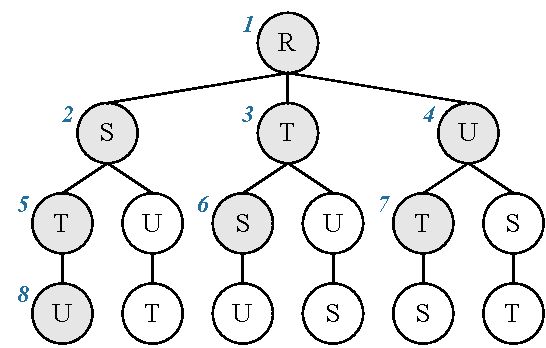
\includegraphics[width=0.5\linewidth]{figures/join_order_search_space-3.pdf}
    \vspace{-0.15cm}
    \caption{The Join Order Search Space as a Tree: A path from root to leaf denotes a sequence of joins. The visited nodes are marked in gray, and the digits indicate the order in which they are visited using the Next-Best Join Order Search. At step 8, the algorithm emits the first join order $\langle R, S, T, U \rangle$.}
    \label{fig:search_space}
    \vspace{-0.35cm}
\end{figure}

\textbf{Basic Heuristics:} Besides the search-based approaches, we use two simple additional heuristics to generate alternative join orders: 
\begin{itemize}
\item \textbf{S3 \textsc{PushDown}:} Permute the original join order such that each join gets pushed to be the first in the join order once if legal (assuming that the first join in the pipeline often has the largest performance impact~\cite{DBLP:conf/damon/SchubertGZM23}).
\item \textbf{S4 \textsc{PullUp}:} Pull each join to the last position in the join order if possible (assuming that join blowups may be mitigated if the problematic join is pulled up to the end of the join order as other joins may filter its input).
\end{itemize}

\subsection{Pipeline Execution}\label{sec:execution}

During query execution, POLAR routes tuples from the source table of a pipeline through multiple join paths. The pipeline executor of these paths reports the performance and calculates their \emph{resistance} for future routing decisions. By using thread-local state (e.g., for tuple buffers and multiplexer state), POLAR can execute its pipelines in parallel without blocking. In this section, we discuss the related techniques for pipeline orchestration, our resistance metric, and parallel execution strategies in detail.

\textbf{Pipeline Orchestration:} To process a POLAR pipeline, the database system spawns a custom POLAR pipeline executor responsible for passing tuples to the operators according to the multiplexer's routing decisions. 
The executor fetches chunks (\ie mini-batches or sets of tuples) from the source and passes them sequentially through the pipeline. The multiplexer consumes a chunk and returns an output chunk containing a subset of the input (or the whole input) and the index of the next join order to pass the subset to. If the multiplexer does not return all tuples from the input, the executor re-invokes the multiplexer with the same input chunk in the next iteration to emit the next tuple subset instead of fetching a new chunk from the source. After routing the chunk to its dedicated join order, the executor passes the chunk to the adaptive union, other pipeline operators, and finally the pipeline sink. During this process, the executor counts the number of intermediates appearing within the path as a performance indicator. We chose intermediates over time because they allow isolated observations (irrespective of other operators and parallelism), and the related $C_{out}$ cost model is known to be simple yet accurate \cite{moerkotte23, LeisGMBK015}. After fully processing one multiplexer output chunk in a join order, the executor reports back the number of intermediates from that routing iteration to the multiplexer. This design allows adapting the \emph{plans of least resistance} to clustered data. For example, table $R$ from Figure~\ref{fig:pipeline_design} may have many matches with $S$ and few with $T$ for its first half of rows but behave the opposite for its second half. For this reason, POLAR never discards previously generated join orders.

\begin{figure}[!b]
    \centering
		\vspace{-0.35cm}
    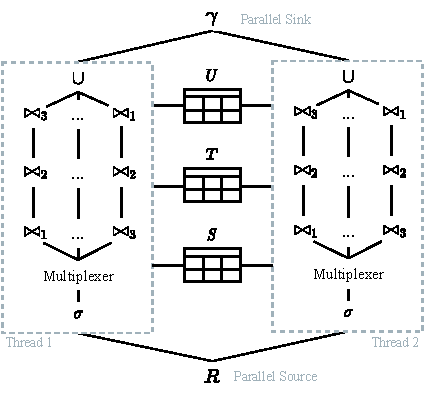
\includegraphics[width=0.82\linewidth]{figures/parallel-exec-2-2.pdf}
    \vspace{-0.5cm}
    \caption{Parallel Execution: Each thread processes a pipeline with an isolated state, sharing build sides to probe into.}
    \vspace{-0.25cm}
    \label{fig:parallel-exec}
\end{figure}

\textbf{Resistance Metric:} As a proxy for performance, the POLAR executor calculates a join order \emph{resistance}. This quantity comprises the sum of intermediate results $I$ observed in the current routing iteration, the number of tuples routed to the current join order $T$, and a constant $w$ representing the overhead of a routing iteration without intermediate results. We calculate the resistance as ${r = \frac{I}{T} + w}$. The constant $w$ prevents edge cases of a routing iteration with zero intermediates counting as infinitely better than an iteration with few intermediates. If only a few tuples are routed to a join order, the resistance may not be representative for a larger set of tuples. Consequently, the executor applies a moving average from previous iterations for smoothing fluctuations.

\textbf{Parallel Execution:} Similar to traditional data-parallel processing, POLAR executes pipelines in a multi-threaded fashion using multiple executors with thread-local states (cf. Figure~\ref{fig:parallel-exec}). The executors concurrently fetch batches of tuples from the source and push results to the sink. Each executor has an isolated multiplexer state and calculates the path resistances solely based on its fetched tuples. Note that the executors only isolate their processing states but share build-side data structures such as read-only hash tables. With the input tuples, the executor follows the paths sequentially and independently from each other. The lack of global multiplexing may delay finding better paths because each multiplexer computes resistances individually. However, this parallelization strategy avoids synchronization among the executors and ensures correct resistance metrics for clustered data. As an alternative baseline parallelization strategy, POLAR also supports spawning one thread per join order and applying a backpressure mechanism to route tuples in a self-scheduling manner (cf. Section~\ref{sec:backpressure}).


%%%%%%%%%%%%%%%%%%%%%%%%%%%%%%%%%%%%%%%%%%%%%%%%%%%%%%%%%%%%%%%%%%%%%%%%%%%%%%%%%%%%
%% ROUTING STRATEGY
%%%%%%%%%%%%%%%%%%%%%%%%%%%%%%%%%%%%%%%%%%%%%%%%%%%%%%%%%%%%%%%%%%%%%%%%%%%%%%%%%%%%


\section{Routing Strategies}
\label{sec:routing_strategies}

At the core of POLAR pipeline execution is the multiplexer operator that makes routing decisions for exploration and exploitation to determine the number of input tuples for each join order. To this end, the pipeline executor passes an input chunk to the multiplexer, which uses a \emph{routing strategy} to return the next join path index and a subset of the tuples to route. The routing strategies attempt to follow the \emph{plans of least resistance}, which is the---potentially temporally changing---sequence of join order paths that incur the fewest number of intermediates. In this section, we first discuss the overall multiplexer algorithm, followed by four dedicated routing strategies used by the multiplexer and one self-scheduling strategy.

%%%%%%%
\subsection{Overall Multiplexer Algorithm}
\label{sec:multiplexer}

Algorithm \ref{alg:multiplexer} shows the overall multiplexer algorithm. In the initialization phase, the multiplexer sends a small number of tuples to each join order with a resistance of zero (\ie an uninitialized join order without reported resistance) to measure initial performance. When all join orders are initialized, the multiplexer requests a tuple distribution from a configurable routing strategy. The distribution indicates the fraction that each join order receives from the current input chunk. The algorithm finally returns the join order index with the largest fraction and its respective input tuple count. If the multiplexer does not emit all tuples from the input chunk, the multiplexer emits the remaining tuples from the tuple distribution in the next iteration until the input chunk is fully processed (cf. Section~\ref{sec:execution}).
%
In the following, we introduce four different routing strategies implementing the tuple distribution method. Assuming that POLAR is executed in a vectorized database system, the implementation must trade-off path optimality (following the cheapest path through the join orders) and operator cache friendliness (minimizing the number of join order switches). The caching aspect can impact the processing performance as the pipeline executor must flush all operator caches buffering intermediates for vectorization before reporting the join order resistance to ensure that each input tuple has been fully processed and was thus correctly counted. Additionally, processing without buffering or too frequent plan switches may increase the number of instruction cache misses~\cite{SirinTPA16}. 

\begin{algorithm}[!t]
\caption{Multiplexer}\label{alg:multiplexer} \small
\begin{algorithmic}[1]
\Require{Tuple Distribution $T$, Resistances $\mat{W}$} 
\Ensure{Join Order Index $\mathit{idx}$, Tuple count $c$}
\If{$\exists t_{\mathit{idx}} \in T: t_{\mathit{idx}} > 0$}
    \State $\mathit{fraction} \gets t_{\mathit{idx}}$ \Comment{Route tuples from previous multiplexing}
    \State $t_{\mathit{idx}} \gets 0$
    \State\Return $\mathit{idx}$, $\mathit{fraction} \cdot \mathit{INPUT\_SIZE}$
\ElsIf{$\exists w_{\mathit{idx}} \in \mat{W}: w = 0$} \Comment{Initialize join order}
    \State\Return $\mathit{idx}$, $\textsc{INIT\_COUNT}$
\EndIf
\State $T \gets \textsc{GetTupleDistribution}(\mat{W})$
\State $\mathit{idx}, \mathit{fraction} \gets \textsc{max}(T)$
\State $t_{\mathit{idx}} \gets 0$
\State\Return $\mathit{idx}$, $\mathit{fraction} \cdot \textsc{INPUT\_SIZE}$
\end{algorithmic}
\end{algorithm}

%%%%%%%
\subsection{Static Selection}

Static routing strategies, or path selection approaches, do not perform any exploration apart from initialization. For this reason, they are very simple to implement, and thus, we omit their pseudo-code of $\textsc{GetTupleDistribution}$ but provide high-level descriptions.

\textbf{R1 \textsc{InitOnce}:} This simple strategy retrieves the join order with the lowest resistance after the initialization phase and then routes every following chunk to that join order. \textsc{InitOnce} is extremely cache-friendly (i.e., in terms of tuple buffering in operator pipelines) because it does not require path switching or counting intermediates throughout the query. However, this strategy is prone to bad routing if a join order only performs well for the first few tuples. Moreover, it is unable to find well-performing paths if different join orders are optimal for different data clusters of the source.

\textbf{R2 \textsc{Opportunistic}:} The \textsc{Opportunistic} routing strategy is similar to \textsc{InitOnce} but makes use of the resistance reports after routing each chunk. If the reported resistance of the current join order exceeds the resistance of another, it routes the next input chunks to that join order. This approach allows switching join orders if the previous order deteriorates. However, the decision is solely based on the resistance of a single join order and old initialization results of others, which may miss additional opportunities, such as better plans for clusters of data. Cache flushing is needed but can be reduced by only updating the resistance after every $n$-th chunk, trading granularity with cache-efficiency.  

%%%%%%%
\subsection{Pro-active Exploration}

\begin{figure*}[!t]
    \centering
    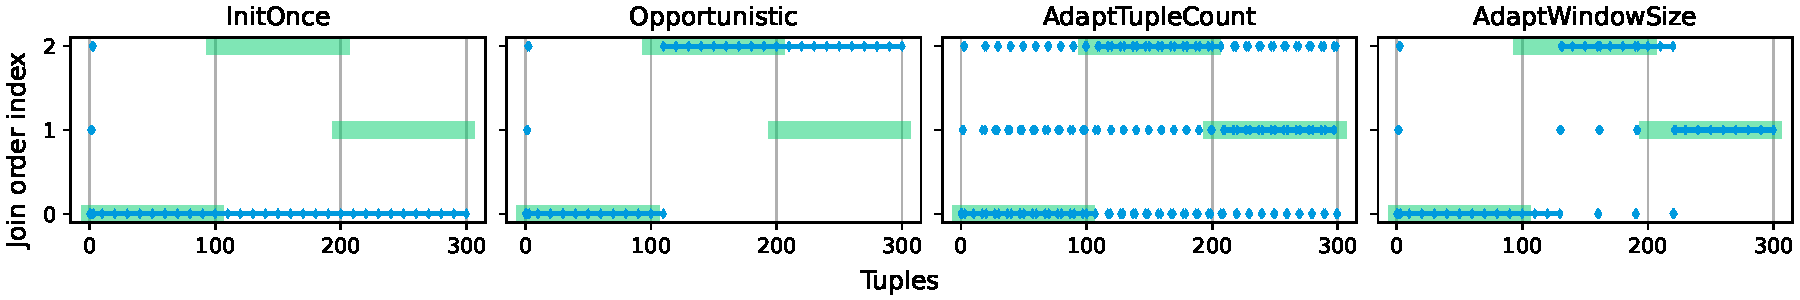
\includegraphics[width=0.99\linewidth]{figures/routing_example.pdf}
		\vspace{-0.2cm}
    \caption{Behavior of four different routing strategies in a single-threaded example scenario with 30 input batches of 10 tuples each (green: optimal join paths, blue diamond: multiplexer invocations, blue line: path chosen by routing strategy).}
    \vspace{-0.1cm}
    \label{fig:routing_example}
\end{figure*}

In order to handle varying data characteristics and find well-per\-form\-ing join orders, routing strategies need to pro-actively explore alternative join orders. To this end, these strategies periodically route tuples to join orders that performed sub-optimal in the past. We introduce two strategies that both use the notion of an \emph{exploration budget} that probabilistically bounds the overhead the strategy allocates for finding the optimal join path (cf. Section~\ref{sec:objectives}). The two following strategies use the exploration budget to calculate a tuple distribution over the join orders, producing additional intermediates based on the resistances measured so far.

\begin{algorithm}[!t] \small
\caption{GetTupleDistribution -- \textsc{AdaptTupleCount}}\label{alg:adapt_tuple_count}
\begin{algorithmic}[1]
\Require{Resistances $\mat{W}$, \textbf{Output:} Tuple Distribution $T$}
%\Ensure{Tuple Distribution $T$}
\State $T \gets \textsc{Initialize}(\card{\mat{W}}, 1)$
\State $\mat{W} \gets \textsc{SortInc}(\mat{W})$
\State $\mathit{cost} \gets \textsc{LastElement}(\mat{W})$
\For{$i \gets \card{\mat{W}} - 1$ \textbf{to} $0$}\Comment{Calculate distribution bottom-up}
    \State $\mathit{target} \gets w_i \cdot (1 + \textsc{BUDGET})$
    \State $\mathit{decrease} \gets \frac{w_i - \mathit{target}}{w_i - \mathit{cost}}$
    \For{$j \gets i+1$ \textbf{to} $\card{\mat{W}}$}\Comment{Adjust fractions to new target}
        \State $t_j \gets t_j \cdot \mathit{decrease}$
    \EndFor
    \State $t_i \gets 1 - \mathit{decrease}$
    \State $\mathit{cost} \gets \mathit{target}$
\EndFor
\State\Return $T$
\end{algorithmic}
\end{algorithm}


\begin{algorithm}[!t] \small
\caption{GetTupleDistribution -- \textsc{AdaptWindowSize}}\label{alg:adapt_window_size}
\begin{algorithmic}[1]
\Require{Resistances $\mat{W}$, \textbf{Output:} Tuple Distribution $T$}
%\Ensure{Tuple Distribution $T$}
\State $T \gets \textsc{Initialize}(\card{\mat{W}}, 0)$
\State $t_{\textsc{minIndex}(W)} \gets 1$ \Comment{Route all tuples to least resistant order}
\State $\mathit{size}$, $\mathit{offset} \gets \textsc{GetWindowState}()$
\If{$\mathit{size} = 0$} \Comment{Determine window size}
    \State $W^{\prime} \gets \mat{W} \setminus \textsc{min}(\mat{W})$
    \State $\mathit{size} \gets \frac{1}{\textsc{INPUT\_SIZE}} \cdot \frac{\sum w^{\prime}_i \cdot \textsc{INIT\_COUNT}}{\textsc{BUDGET} \cdot \textsc{min}(W)}$
\EndIf
\If{$\mathit{offset} < \mathit{size}$}
    \State $\mathit{offset} \gets \mathit{offset} + 1$
\Else \Comment{Re-explore join orders next time}
    \State $\mat{W} \gets \textsc{SetToZero}(\mat{W} \setminus \textsc{min}(\mat{W}))$ \Comment{Reset resistances}
    \State $\mathit{offset}, \mathit{size} \gets 0$
\EndIf
\State $\textsc{SetWindowState}(\mathit{size}, \mathit{offset})$
\State\Return $T$
\end{algorithmic}
\end{algorithm}

\textbf{R3 \textsc{AdaptTupleCount}:} For each input chunk, the \textsc{AdaptTupleCount} strategy determines a tuple distribution that (assuming previous resistances) would stay within the exploration budget relative to the best path's intermediate count.
%
The strategy initializes the output tuple fractions with ones (line 1), orders paths by their resistances (line 2), and adjusts the distribution in a bottom-up fashion. We start by reducing the problem to the two join orders with the highest resistances. The target cost is based on the lower resistance and the exploration budget, which we then use to calculate a \textit{decrease} factor (line 6). By multiplying that factor with the join order's tuple fraction, we find the amount of tuples that must be sent to the worst join order to stay within the exploration budget based on the resistance of the second-last join order. Consequently, the amount for the second-last order is $1 - \mathit{decrease}$ (line 10). We calculate these values for the next-best join order while decreasing the fractions of the orders with higher resistances until we reach the first join order. \textsc{AdaptTupleCount} calculates tuple distributions for each incoming chunk, allowing for fine-grained path exploration bounded by the exploration budget. However, splitting each chunk into smaller sets of tuples obstructs vectorized execution and causes many cache flushes to report resistances. To reduce the number of splits per chunk, the algorithm could serve only join orders receiving more than $n$ tuples, redistributes unserved tuples, and recalls them when calculating the next distribution.

\textbf{R4 \textsc{AdaptWindowSize}:} In contrast to \textsc{AdaptTupleCount}, the \textsc{AdaptWindowSize} strategy does not calculate individual tuple counts per join order. Instead, this strategy either routes complete chunks or a static, low number of tuples and adapts the window size (\ie number of input chunks) within which it will only serve the best join order. When exceeding the window, it re-initializes the remaining join orders by routing a small number of tuples to each of them. The internals of this strategy are shown in Algorithm~\ref{alg:adapt_window_size}, which distinguishes between three cases. Irrespective of the case, this strategy always returns a tuple distribution in which the best order receives the whole input chunk (line 2). If there is no window size calculated yet (line 4), we estimate the number of intermediates occurring in a reinitialization phase based on the resistances and adjust the number of tuples for reinitialization accordingly. We then divide the cost estimate by the overhead allowed by the exploration budget resulting in the number of tuples that should be routed to the best join order before reinitializing the others. The number of tuples per chunk scales this value down to the window size (line 6). If the current offset does not exceed the window size, we increment it (line~9). Finally, if the window size is exceeded, we set the resistances for all join orders, except the best, to zero (line 12) to trigger re-initialization on the next invocation. By routing multiple chunks to the same join order, the \textsc{AdaptWindowSize} strategy better allows for vectorization and can defer cache flushing until the window size is exceeded. On the other hand, its path exploration granularity is more coarse-grained than \textsc{AdaptTupleCount} as changes in resistances may appear within the routing window.

\begin{example2}[Routing Example] To illustrate the behavior of the routing strategies, Figure \ref{fig:routing_example} compares their  decisions in an example scenario (three join orders, 30 input chunks of 10 tuples each). The resistances of the join orders change every 10 chunks, namely $C_0 \gets \langle 1, 10, 15 \rangle$, $C_{10} \gets \langle 10, 15, 5 \rangle$, and $C_{20} \gets \langle 10, 1, 5 \rangle$. The resulting optimal path changes from 1st to 3rd to 2nd (indicated as green solid lines). The blue diamonds show the multiplexer invocations of the different paths, and the blue line indicates the chosen path. \textsc{Init\-Once} tests every join order once and follows the initially optimal path. The \textsc{Opportunistic} strategy switches to the correct path after the first one deteriorates but misses the second switch. \textsc{AdaptTupleCount} correctly adapts to the optimal join paths but requires many switches and multiplexer invocations, including cache flushing. Finally, \textsc{AdaptWindowSize} first uses a large window and thus detects the join order switch only after a delay. Later, it reduces the window size as the difference between the resistances decreases. Hence, the next switch comes after a shorter delay due to window resizing.
\end{example2}

\subsection{Self-scheduling}\label{sec:backpressure}

\textbf{R5 \textsc{Backpressure}:} To enable comparing against a self-scheduling strategy without parameters, we include a \enquote{backpressure} strategy. Instead of using a multiplexer, the POLAR pipeline spawns individual threads for each join order so that each thread concurrently pulls new input chunks. The approach does not depend on a budget and simply favors faster join orders as they can pull more chunks per time unit than others. The \textsc{Backpressure} strategy does not rely on multiplexing, does not require any operator cache flushes, and thus, fully supports vectorized execution. However, with potentially many join orders, this strategy has the intrinsic limitation that the majority of threads waste CPU cycles on sub-optimal paths.

%%%%%%%%%%%%%%%%%%%%%%%%%%%%%%%%%%%%%%%%%%%%%%%%%%%%%%%%%%%%%%%%%%%%%%%%%%%%%%%%%%%%
%% LIMITATIONS
%%%%%%%%%%%%%%%%%%%%%%%%%%%%%%%%%%%%%%%%%%%%%%%%%%%%%%%%%%%%%%%%%%%%%%%%%%%%%%%%%%%%

\section{Limitations and Scope}
\label{sec:limits}
%
POLAR is designed for adaptive query processing with non-invasive system integration as well as small and bounded overhead. This design leads to certain limitations as its applicability is ultimately dependent on the system's existing query optimizer. 
\begin{itemize}
\item \emph{Amenable Pipelines:} POLAR only replaces left-deep-trees. If the optimizer emits a right-deep tree (where intermediates feed into the build side of hash joins), POLAR cannot generate alternative join orders, as there are no pipelines with more than one join. Support for directed acyclic graphs (DAGs) and bushy trees is interesting future work.
\item \emph{Source Table:} As POLAR replaces normal operator pipelines that consume tuples from a specific source, it cannot change the source (sometimes called driver \cite{LiSMBCL07}) table.
\item \emph{Operator Types:} POLAR only supports pipelines with join sequences. Extended support for additional operators---such as projection, selection, and groupjoin \cite{MoerkotteN11}---is interesting future work as well.
\end{itemize}
%
POLAR is currently most applicable to star-schema workloads with cardinality estimation challenges (\eg parameterized queries, UDFs, correlated data). If the source table contains clustered data (\eg orders sorted by date with different join cardinalities over time), POLAR can further exploit different plans for different data.